\section{Results}
The central empirical finding is consistent across model scale, graph domain, and comparison method - profile and trace conditioning make trajectories easier to analyze, but they do not improve final ranking in this implementation.

\subsection{Validation ablation: profile and trace conditioning hurt MRR}
Table~\ref{tab:validation} reports the Qwen3-14B validation ablation averaged across PRIME, MAG, and Amazon. The ``Steps'' column is the maximum number of action-observation iterations allowed before final-answer emission. The metric columns are averages across the three graphs. The unconditioned agent with a 12-step budget obtains the best average \mrr (.4087), while the complete \tb agent obtains .3141 at 12 steps and .3103 at 16 steps. The profile-only and trace-only variants also underperform the unconditioned agent, showing that the degradation is not caused by only one component.

\begin{table}[t]
\centering
\caption{\textbf{Validation ablation averaged over PRIME, MAG, and Amazon.} The unconditioned agent is strongest, while the combined \tb agent loses both rank precision and recall.}
\label{tab:validation}
\resizebox{\columnwidth}{!}{%
\begin{tabular}{lrrrrr}
\toprule
Controller variant & Steps & \hit{1} & \hit{5} & \recall{20} & \mrr \\
\midrule
Unconditioned agent & 12 & \textbf{.3333} & \textbf{.5100} & \textbf{.4252} & \textbf{.4087} \\
 & 16 & .3233 & .5067 & .4192 & .4058 \\
\midrule
Profile-only agent & 12 & .2833 & .4533 & .3845 & .3511 \\
 & 16 & .2533 & .4700 & .3848 & .3473 \\
\midrule
Trace-only agent & 12 & .2333 & .3767 & .2840 & .2944 \\
 & 16 & .2733 & .4167 & .3195 & .3307 \\
\midrule
\tb agent & 12 & .2579 & .3951 & .3036 & .3141 \\
 & 16 & .2567 & .3900 & .2998 & .3103 \\
\bottomrule
\end{tabular}}
\end{table}

\begin{figure}[t]
\centering
\resizebox{\columnwidth}{!}{\providecolor{mplblue}{HTML}{1F77B4}

\begin{tikzpicture}
\begin{axis}[
    width=6.9in,
    height=3.15in,
    ybar,
    bar width=0.66cm,
    ymin=0,
    ymax=0.46,
    ylabel={Mean Reciprocal Rank},
    xtick={1,2,3,4,5,6,7,8},
    xticklabels={
        {Uncond.\\12},
        {Uncond.\\16},
        {Profile\\12},
        {Profile\\16},
        {Trace\\12},
        {Trace\\16},
        {TraceBound\\12},
        {TraceBound\\16}
    },
    xticklabel style={align=center,font=\large},
    xmin=0.4,
    xmax=8.6,
    ytick={0.0,0.1,0.2,0.3,0.4},
    tick label style={font=\large},
    label style={font=\Large},
    title style={font=\LARGE},
    axis x line*=bottom,
    axis y line*=left,
    axis line style={black,semithick},
    tick style={black},
    nodes near coords={
        \pgfmathprintnumber[fixed,precision=3,zerofill]{\pgfplotspointmeta}
    },
    point meta=rawy,
    every node near coord/.append style={
        font=\normalsize,
        black,
        anchor=south,
        yshift=2pt
    },
    clip=false,
]
\addplot+[fill=mplblue,draw=mplblue] coordinates {
    (1,0.409)
    (2,0.406)
    (3,0.351)
    (4,0.347)
    (5,0.294)
    (6,0.331)
    (7,0.314)
    (8,0.310)
};

\draw[mplblue,dashed,thick]
    (axis cs:0.35,0.409) -- (axis cs:8.65,0.409);

\node[anchor=west,font=\normalsize]
    at (axis cs:3.45,0.426)
    {best unconditioned baseline};

\end{axis}
\end{tikzpicture}
}
\caption{\textbf{Validation MRR by controller variant and step budget.} The dashed horizontal reference line marks the best unconditioned baseline. All profile/trace variants fall below that line, so the intervention improves neither the 12-step nor the 16-step validation setting.}
\label{fig:validation_mrr}
\end{figure}

\subsection{Held-out subset: the direction persists with a stronger controller}
Table~\ref{tab:heldout} reports the Qwen3-30B-A3B held-out subset. The ``$n$'' column is the number of completed examples in that graph and condition. The pattern is again negative for \tb. On MAG, the most severe case, \tb reduces \mrr from .7711 to .4974. PRIME and Amazon have smaller but still negative changes. This matters because MAG is the graph where relation-rich academic queries can strongly reward precise anchoring; misdirected adaptive exploration can therefore move the controller toward plausible but wrong neighborhoods.



\begin{figure}[t]
\centering
\resizebox{\columnwidth}{!}{\providecolor{mplblue}{HTML}{1F77B4}
\providecolor{mplorange}{HTML}{FF7F0E}
\providecolor{mplgreen}{HTML}{2CA02C}

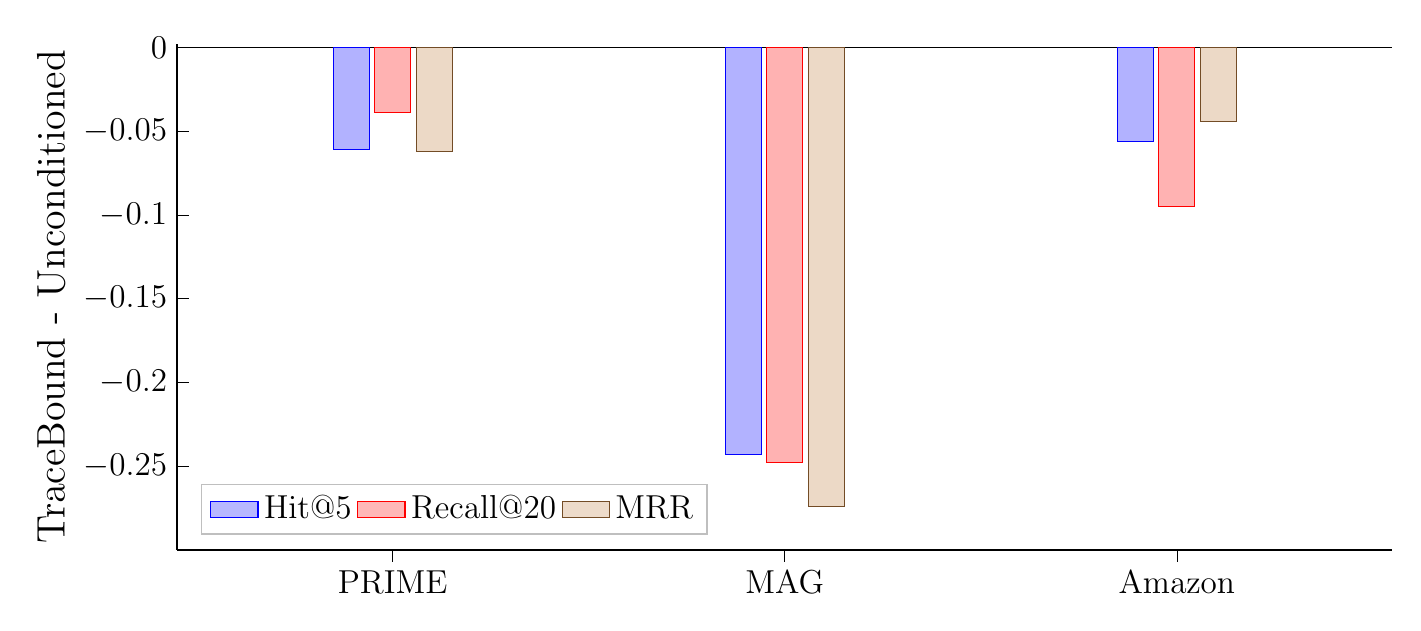
\begin{tikzpicture}
\begin{axis}[
    width=6.7in,
    height=3.15in,
    ybar,
    area legend,
    bar width=13pt,
    ymin=-0.3,
    ymax=0.002,
    xmin=0.45,
    xmax=3.55,
    ylabel={TraceBound - Unconditioned},
    xtick={1,2,3},
    xticklabels={PRIME,MAG,Amazon},
    ytick={0,-0.05,-0.10,-0.15,-0.20,-0.25},
    yticklabel style={/pgf/number format/fixed,/pgf/number format/precision=2},
    xticklabel style={font=\large},
    tick label style={font=\large},
    label style={font=\Large},
    title style={font=\LARGE},
    axis x line*=bottom,
    axis y line*=left,
    axis line style={black,semithick},
    tick style={black},
    extra y ticks={0},
    extra y tick labels={},
    extra y tick style={
        grid=major,
        major grid style={black,semithick},
        tick style={draw=none}
    },
    legend style={
        at={(0.02,0.03)},
        anchor=south west,
        draw=gray!50,
        fill=white,
        fill opacity=0.92,
        text opacity=1,
        legend columns=3,
        font=\large
    },
    legend cell align={left},
]
\addplot+[] coordinates {
    (1,-0.061)
    (2,-0.243)
    (3,-0.056)
};
\addplot+[] coordinates {
    (1,-0.039)
    (2,-0.248)
    (3,-0.095)
};
\addplot+[] coordinates {
    (1,-0.062)
    (2,-0.274)
    (3,-0.044)
};
\legend{Hit@5, Recall@20, MRR}
\end{axis}
\end{tikzpicture}
}
\caption{\textbf{Held-out metric deltas.} Each grouped bar is \tb minus unconditioned on the held-out subset. Bars below zero mean the profile/trace intervention is worse. The three bars per graph correspond to \hit{5}, \recall{20}, and \mrr; all are negative across PRIME, MAG, and Amazon.}
\label{fig:heldout_delta}
\end{figure}

\begin{table}[t]
\centering
\caption{\textbf{Held-out subset with Qwen3-30B-A3B.} Each row is one graph-condition cell. ``$n$'' gives completed examples. The \tb rows underperform the corresponding unconditioned rows on every graph.}
\label{tab:heldout}
\resizebox{\columnwidth}{!}{%
\begin{tabular}{llrrrrr}
\toprule
Graph & Controller & $n$ & \hit{1} & \hit{5} & \recall{20} & \mrr \\
\midrule
PRIME & Unconditioned & 290 & .2966 & .4207 & .3681 & .3499 \\
 & \tb & 300 & .2400 & .3600 & .3297 & .2880 \\
\midrule
MAG & Unconditioned & 299 & .7224 & .8328 & .7483 & .7711 \\
 & \tb & 300 & .4233 & .5900 & .5006 & .4974 \\
\midrule
Amazon & Unconditioned & 296 & .5439 & .7128 & .4557 & .6152 \\
 & \tb & 300 & .5033 & .6567 & .3607 & .5714 \\
\bottomrule
\end{tabular}}
\end{table}

\subsection{Paired comparison: the result is not an artifact of completed-count differences}
Table~\ref{tab:paired} keeps only shared query IDs available in both unconditioned and \tb outputs. ``Paired $n$'' is the number of shared examples. Each delta is \tb minus unconditioned on the same queries. The paired comparison confirms the aggregate result: all reported deltas are negative. MAG again shows the largest effect, with a -.2711 paired \mrr delta.

\begin{table}[t]
\centering
\caption{\textbf{Shared-ID paired diagnostics.} Rows compare \tb and the unconditioned agent on identical query IDs. $\Delta\hit{5}$, $\Delta\recall{20}$, and $\Delta\mrr$ are \tb-minus-unconditioned. Negative values indicate that \tb ranks correct answers lower or retrieves fewer gold answers.}
\label{tab:paired}
\resizebox{0.85\columnwidth}{!}{%
\begin{tabular}{lrrrr}
\toprule
Graph & Paired $n$ & $\Delta\hit{5}$ & $\Delta\recall{20}$ & $\Delta\mrr$ \\
\midrule
PRIME & 291 & -.0653 & -.0421 & -.0653 \\
MAG & 300 & -.2400 & -.2452 & -.2711 \\
Amazon & 297 & -.0539 & -.0911 & -.0426 \\
\bottomrule
\end{tabular}}
\end{table}

\subsection{Effect-size summary}
Across the three held-out graphs, the average paired \mrr delta is negative. The magnitude is not uniform. MAG accounts for the largest drop, PRIME is moderate, and Amazon is smaller but still negative. This heterogeneity is scientifically useful: it shows that adaptive failure depends on graph structure and query type. A controller that can recover on product queries may still fail badly on academic graph queries where relation neighborhoods are dense and plausible distractors are common.

